\documentclass[14pt,a4paper]{extarticle}
\usepackage[utf8]{inputenc}

\usepackage[english,russian]{babel}
\usepackage{indentfirst}
\usepackage{amsmath}
\usepackage{amsfonts}
\usepackage{amssymb}
\usepackage{color}
\usepackage{float}
\usepackage{placeins}
\usepackage{mathrsfs}

\numberwithin{equation}{section}


\usepackage[version=3]{mhchem}% Package for chemical equation typesetting
%\renewcommand{\thefigure}{\thechapter.\Alph{figure}}


\usepackage{lineno}

%\linenumbers

\usepackage[usenames,dvipsnames,svgnames,table]{xcolor}
\usepackage[hypcap]{subcaption}
% \usepackage[colorlinks=true, linkcolor=Maroon, citecolor=ForestGreen]{hyperref}
\usepackage[colorlinks=false]{hyperref}
\usepackage{graphicx}
\usepackage{subcaption}
\usepackage[height=25cm, a4paper, hmargin={2.5cm, 1.5cm}, vmargin={2cm, 2.3cm}]{geometry}
\setlength{\parindent}{1em}
\setlength{\parskip}{0pt}% {.3em}

\usepackage{titlesec}
\titleformat*{\section}{\normalsize\bfseries}
\titleformat*{\subsection}{\normalsize\bfseries}
%\titlelabel{\thetitle.\quad}


\usepackage[separate-uncertainty = true, multi-part-units=single, range-phrase=--, range-units=single]{siunitx}

%\mathchardef\period=\mathcode`.
%\DeclareMathSymbol{.}{\mathord}{letters}{"3B}

\usepackage{setspace}
\onehalfspacing

\usepackage[backend=bibtex, style=numeric, sorting=none, maxnames=3, minnames=3, hyperref=true, url=true, isbn=false, backref=true]{biblatex}
\bibliography{mybib}

\usepackage{tocloft}
\usepackage{tikz}
\hyphenation{Ha-ma-ma-tsu}

%\newcommand{\RNum}[1]{\uppercase\expandafter{\romannumeral #1\relax}}

\usepackage{titletoc}
\dottedcontents{section}[3em]{}{2.9em}{1pc}
\dottedcontents{subsection}[3em]{}{2.3em}{1pc}
%\renewcommand{\thesection}{\thechapter\arabic{section}}
%\renewcommand{\thesection}{\thechapter\arabic{subsection}.}

\renewcommand{\figurename}{Рис.}
%\usepackage[labelsep=period, font=small]{caption}

\usepackage{titlesec}
\usepackage{physics}
\titlespacing*{\section}
{0pt}{1pt}{0pt}
% {0pt}{5.5ex plus 1ex minus .2ex}{4.3ex plus .2ex}
\titlespacing*{\subsection}
{0pt}{1pt}{0pt}
% {0pt}{5.5ex plus 1ex minus .2ex}{4.3ex plus .2ex}

\usepackage{fancyhdr}

\pagestyle{fancy}
\fancyhf{}
%\fancyhead[LE,RO]{Share\LaTeX}
%\fancyhead[RE,LO]{Guides and tutorials}
%\fancyfoot[CE,CO]{\leftmark}
\fancyfoot[LE,RO]{\thepage}
\renewcommand{\headrulewidth}{0pt}
\DeclareMathOperator{\sinc}{sinc}

\usepackage{datatool}
\usepackage{siunitx}
\usepackage{booktabs} % for nicer tables
\usepackage{caption} % improve caption spacing (among other things)
\usepackage{bm}
\renewcommand*\dtldisplaystarttab{\toprule}
\renewcommand*\dtldisplayendtab{\tabularnewline\bottomrule}
\renewcommand*\dtldisplayafterhead{\midrule}

\usepackage{pgfplotstable}
\usepackage{siunitx}
\usepackage{booktabs}

\begin{document}

\section{Отчёт по техническому заданию для станции 1-1. Итерация 1.}
\subsection{Входные параметры моделирования}

\subsection{Задача №1}
\textit{Источник - СП ондулятор (параметры ондулятора во вложении, параметры электронного пучка актуализировать у отв. лиц). Оценить размеры и расходимость источника для рабочих гармоник (11-й, 13-й, 17-й и 23-й)}\\
См. рис.~\ref{fig:before_crystal}
При параметрах электронного пучка\\
\begin{table}[h!]
	\centering
	\begin{tabular}{cccccccc}
		\hline
		\toprule
		\rule{0pt}{3ex}   $\sigma_x, [m]$ & $\sigma_{x'}, [rad]$ & $\sigma_y, [m]$     & $\sigma_{y'}, [rad]$ \\ \hline
		\rule{0pt}{3ex}   $33.0 \times 10^{-6}$  & $2.65 \times 10^{-6}$  &  $8.6 \times 10^{-7}$ & $5.0 \times 10^{-7}$   \\
		\hline	\hline
		\rule{0pt}{3ex}   $\Delta E / E$ & $\beta_x,[m]$ & $\beta_y,[m]$   & $I,[mA]$\\ \hline
		\rule{0pt}{3ex}	 $8.6 \times 10^{-4}$ & $12.49$ & $1.99$ & $400$ \\ \hline
		\toprule
		\rule{0pt}{4ex}
	\end{tabular}
	\caption{Пространственные и угловые размеры электронного пучка. Бета функция. Ток}
\end{table}


\DTLloaddb
[
	noheader,
	keys={},
    headers={
    \shortstack{$n_{harm}$},
	\shortstack{$\sigma_x, [mm]$},
	\shortstack{$\sigma_y, [mm]$},
	\shortstack{$\sigma_x, [\mu rad]$},
	\shortstack{$\sigma_y, [\mu rad]$}}
	]
	{RMS_before}{tabl/RMS_before.csv}
\begin{table}[h!]
	\sisetup{
	    parse-numbers   = false,
		table-number-alignment = right,
		table-figures-integer = 4,
		table-figures-decimal = 4,
		input-decimal-markers = .5
	}
	\renewcommand*\dtlrealalign{S}
	\caption{Сечение пучка на входе в первую апертуру (25 м)}
	\centering
	\DTLdisplaydb{RMS_before}
\end{table}

\subsection{Задача №2}
\textit{До первого окна пучок ограничивается прямоугольной апертурой, соответствующей $4\sigma$ сечения пучка по горизонтали и вертикали (рассчитать).}

Здесь лучше писать ориентировать на угловой акцептанс первого кристалла (кривая Дарвина). На рис.~\ref{fig:bragg_R} показаны отражающие способности кристаллов при указанных энергиях. На 14.4 кэВ, ширина кривой $\approx 14 \mu rad$, как видно, 11 гармоника с RMS 3.9 при $4\sigma$ не войдёт в акцептант, оставшаяся часть будет греть кристалл.\\
\textbf{Расстояние от источника}: $25m$\\
\textbf{Апертура}: $0.25mm \times 0.25mm$\\
\textbf{Угловой размер апертуры}: $10\mu rad \times  10 \mu rad$ 

\begin{figure}[htbp]
	\centering  
	\begin{minipage}{0.49\textwidth}
		\centering
		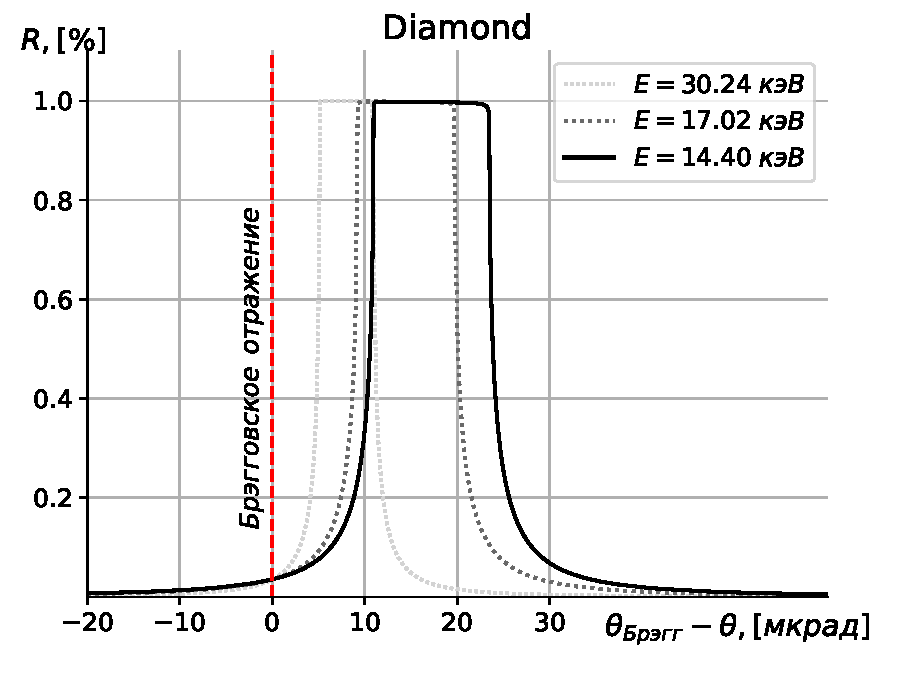
\includegraphics[width=\textwidth]{pic/Diamond_bragg_R.pdf}
		\caption{}
		\label{fig:bragg_R}
	\end{minipage}\hfill
	\begin{minipage}{0.49\textwidth}
		\centering
		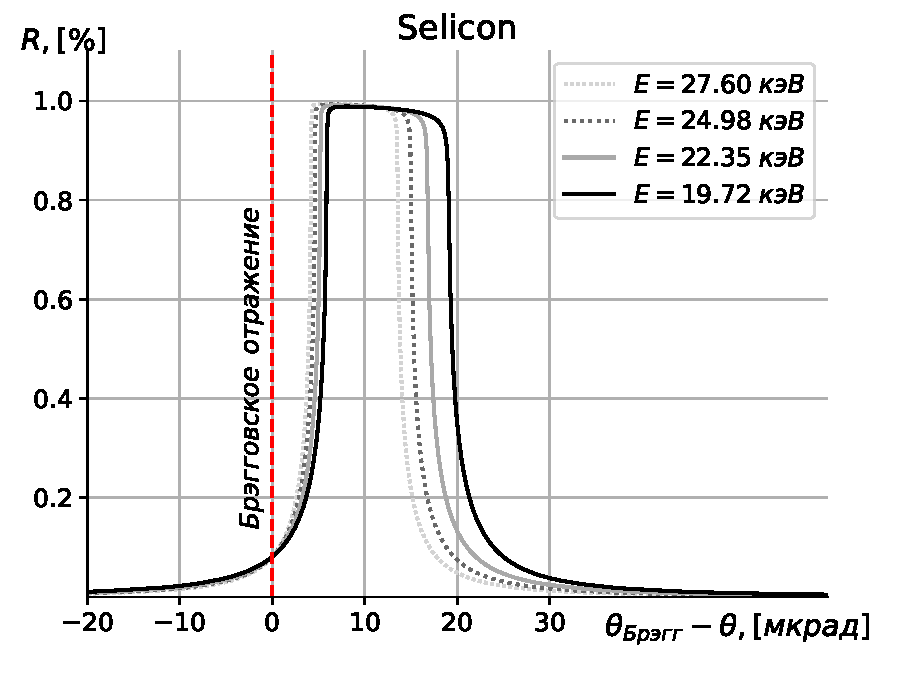
\includegraphics[width=\textwidth]{pic/Selicon_bragg_R.pdf}
		\caption{}
		\label{fig:bragg_T}
	\end{minipage}    
	\begin{minipage}{1.\textwidth}
		\centering  
		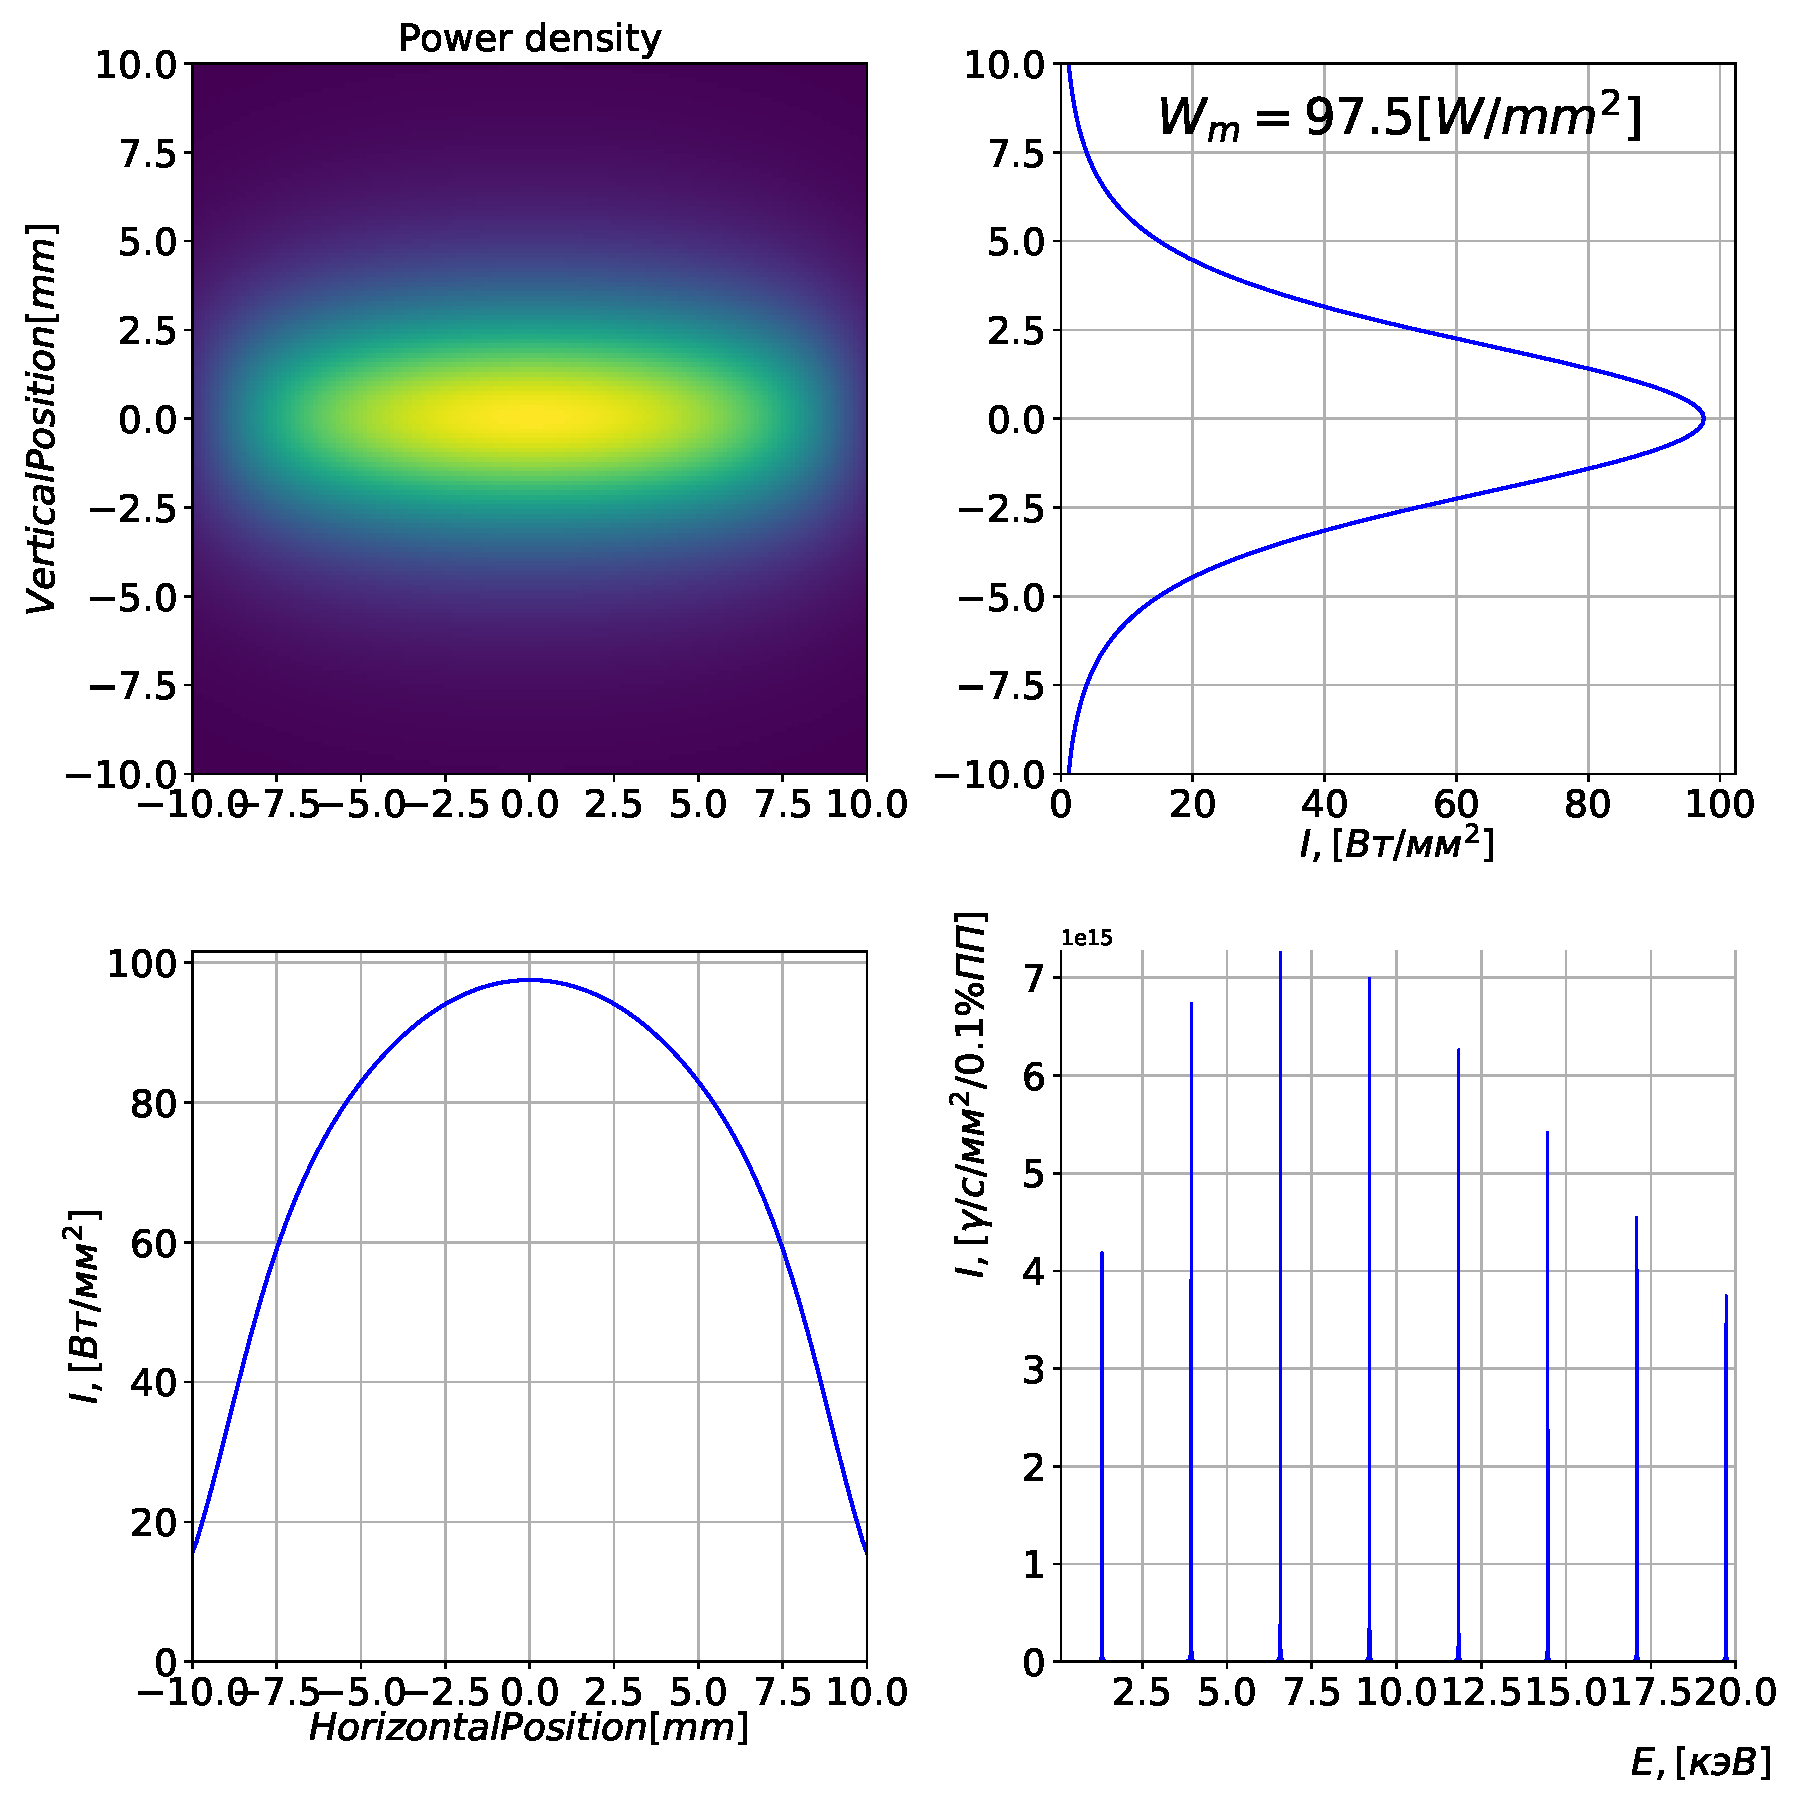
\includegraphics[width=\textwidth]{pic/power_dens.pdf}
		\caption{}
		\label{fig:spec}
\end{minipage}     
\end{figure}

\subsection{Задача №3}
\textit{Далее до выхода из фронт-энда пучок проходит через алмазные окна. Рассчитать суммарную толщину окон из расчёта 1\% подавления первой рабочей гармоники 14,4 кэВ, тепловую мощность, рассеиваемую на окнах, оценить необходимость охлаждения окон.}\\
Кривые поглощения см.рис~\ref{fig:bragg_T}.\\
\textbf{Толщина окна:} $100\mu m$\\
\textbf{Пропускание на 11-ой гармонике:} $T = 0.974 \%$\\
\begin{figure}[htbp]
	\centering  
	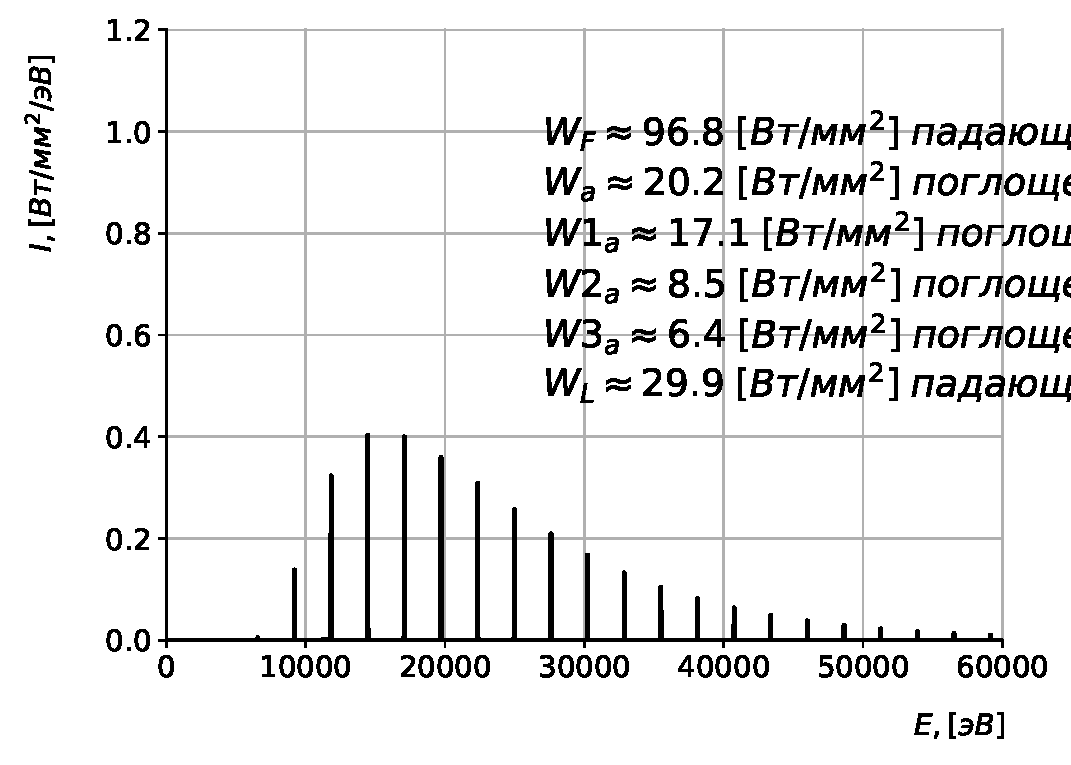
\includegraphics[width=\textwidth]{pic/spec.pdf}
	\caption{Розовый цвет --- падающий на алмазное окно спектр. 
		%Красные и синие отрезки --- потерянная мощность при прохождении пустого промежутка кристалл, 
		чёрные отрезки --- падающий спектр на DCM. Эффективные толщины алмазных монохроматоров: $480.0 [\mu m]$, 11-ая; $568.0 [\mu m]$, 13-ая; $742.0 [\mu m]$, 17-ая; $1004.0 [\mu m]$, 23-ая}
	\label{fig:absorb_spec}
	
\end{figure}


\subsection{Задача №4}
\textit{Непосредственно за стеной фронт-энда (её положение актуализировать у отв. лиц) располагается оптический хатч, в котором максимально близко к фронт-энду (примерная схема во вложении) стоят подряд три алмазных бимсплиттера-монохроматора (Брэгг 111, толщина 100 мкм), отводящих в стороны пучки 11-й, 13-й и 23-й гармоник. Оценить размеры проекции пучка на рабочие поверхности монохроматоров, а также тепловую нагрузку и необходимость охлаждения.}\\
\textbf{Пустые промежутки между кристаллами:} $1m$\\
Тепловые нагрузки см. на рис.~\ref{fig:absorb_spec}\\
Ниже приведены значения поперечных сечений пучка, значения проекций, а также эффективные толщины кристаллов алмазных монохроматоров\\
11 harmonic  $angle =  -77.98 [deg]$ at energy $14461.0$ eV\\ 
$\sigma_x =  0.11 [mm]$\\ 
$\sigma_y =  0.079 [mm]$\\ 
$proj_x  =  0.527 [mm]$\\ 
$Cr_{effective}  =  480.0 [\mu m]$\\
13 harmonic  $angle =  -79.85 [deg]$ at energy $17091.0$ eV\\ 
$\sigma_x =  0.11 [mm]$\\ 
$\sigma_y =  0.08 [mm]$\\ 
$proj_x  =  0.622 [mm]$\\ 
$Cr_{effective}  =  568.0 [\mu m]$\\
17 harmonic  $angle =  -82.26 [deg]$ at energy $22350.0$ eV\\ 
$\sigma_x =  0.108 [mm]$\\ 
$\sigma_y =  0.084 [mm]$\\ 
$proj_x  =  0.8 [mm]$\\ 
$Cr_{effective}  =  742.0 [\mu m]$\\
23 harmonic  $angle =  -84.28 [deg]$ at energy $30238.0$ eV\\ 
$\sigma_x =  0.109 [mm]$\\ 
$\sigma_y =  0.095 [mm]$\\ 
$proj_x  =  1.096 [mm]$\\ 
$Cr_{effective}  =  1004.0 [\mu m]$\\



\subsection{Задача №5}
\textit{Рассчитать сечение пучков, покидающих алмазные монохроматоры.}\\
См.рис.~\ref{fig:after_crystal}

\DTLloaddb
[
noheader,
keys={},
headers={
	\shortstack{$n_{harm}$},
	\shortstack{$\sigma_x, [mm]$},
	\shortstack{$\sigma_y, [mm]$},
	\shortstack{$\sigma_x, [\mu rad]$},
	\shortstack{$\sigma_y, [\mu rad]$}}
]
{RMS_after}{tabl/RMS_after.csv}
\begin{table}[h!]
	\sisetup{
		parse-numbers   = false,
		table-number-alignment = right,
		table-figures-integer = 4,
		table-figures-decimal = 4,
		input-decimal-markers = .5
	}
	\renewcommand*\dtlrealalign{S}
	\caption{Сечение пучка}
	\centering
	\DTLdisplaydb{RMS_after}
\end{table}

\subsection{Задача №5}
\textit{Рассчитать тепловую нагрузку оставшегося прямого пучка на двукристальный кремниевый 111 монохроматор, расположенный в удалённом хатче (см. схему), а также сечение пучка на выходе из монохроматора. Оценить необходимость и тип охлаждения.}\\
Тепловые нагрузки см. на рис.~\ref{fig:absorb_spec}.

\DTLloaddb
[
noheader,
keys={},
headers={
	\shortstack{$n_{harm}$},
	\shortstack{$E, eV$},
	\shortstack{$\lambda, [nm]$},
	\shortstack{$ph/s$},
	\shortstack{$ph/s/0.1\%$}}
]
{ph_beam_par_after_cr}{tabl/ph_beam_par_after_cr.csv}
\begin{table}[h!]
	\sisetup{
		parse-numbers   = false,
		table-number-alignment = right,
		table-figures-integer = 4,
		table-figures-decimal = 4,
		input-decimal-markers = .5
	}
	\renewcommand*\dtlrealalign{S}
	\caption{Сечение пучка на входе в первую апертуру (25 м)}
	\centering
	\DTLdisplaydb{ph_beam_par_after_cr}
\end{table}

\begin{figure}[htbp]
	\centering  
	\begin{minipage}{0.49\textwidth}
		\centering
		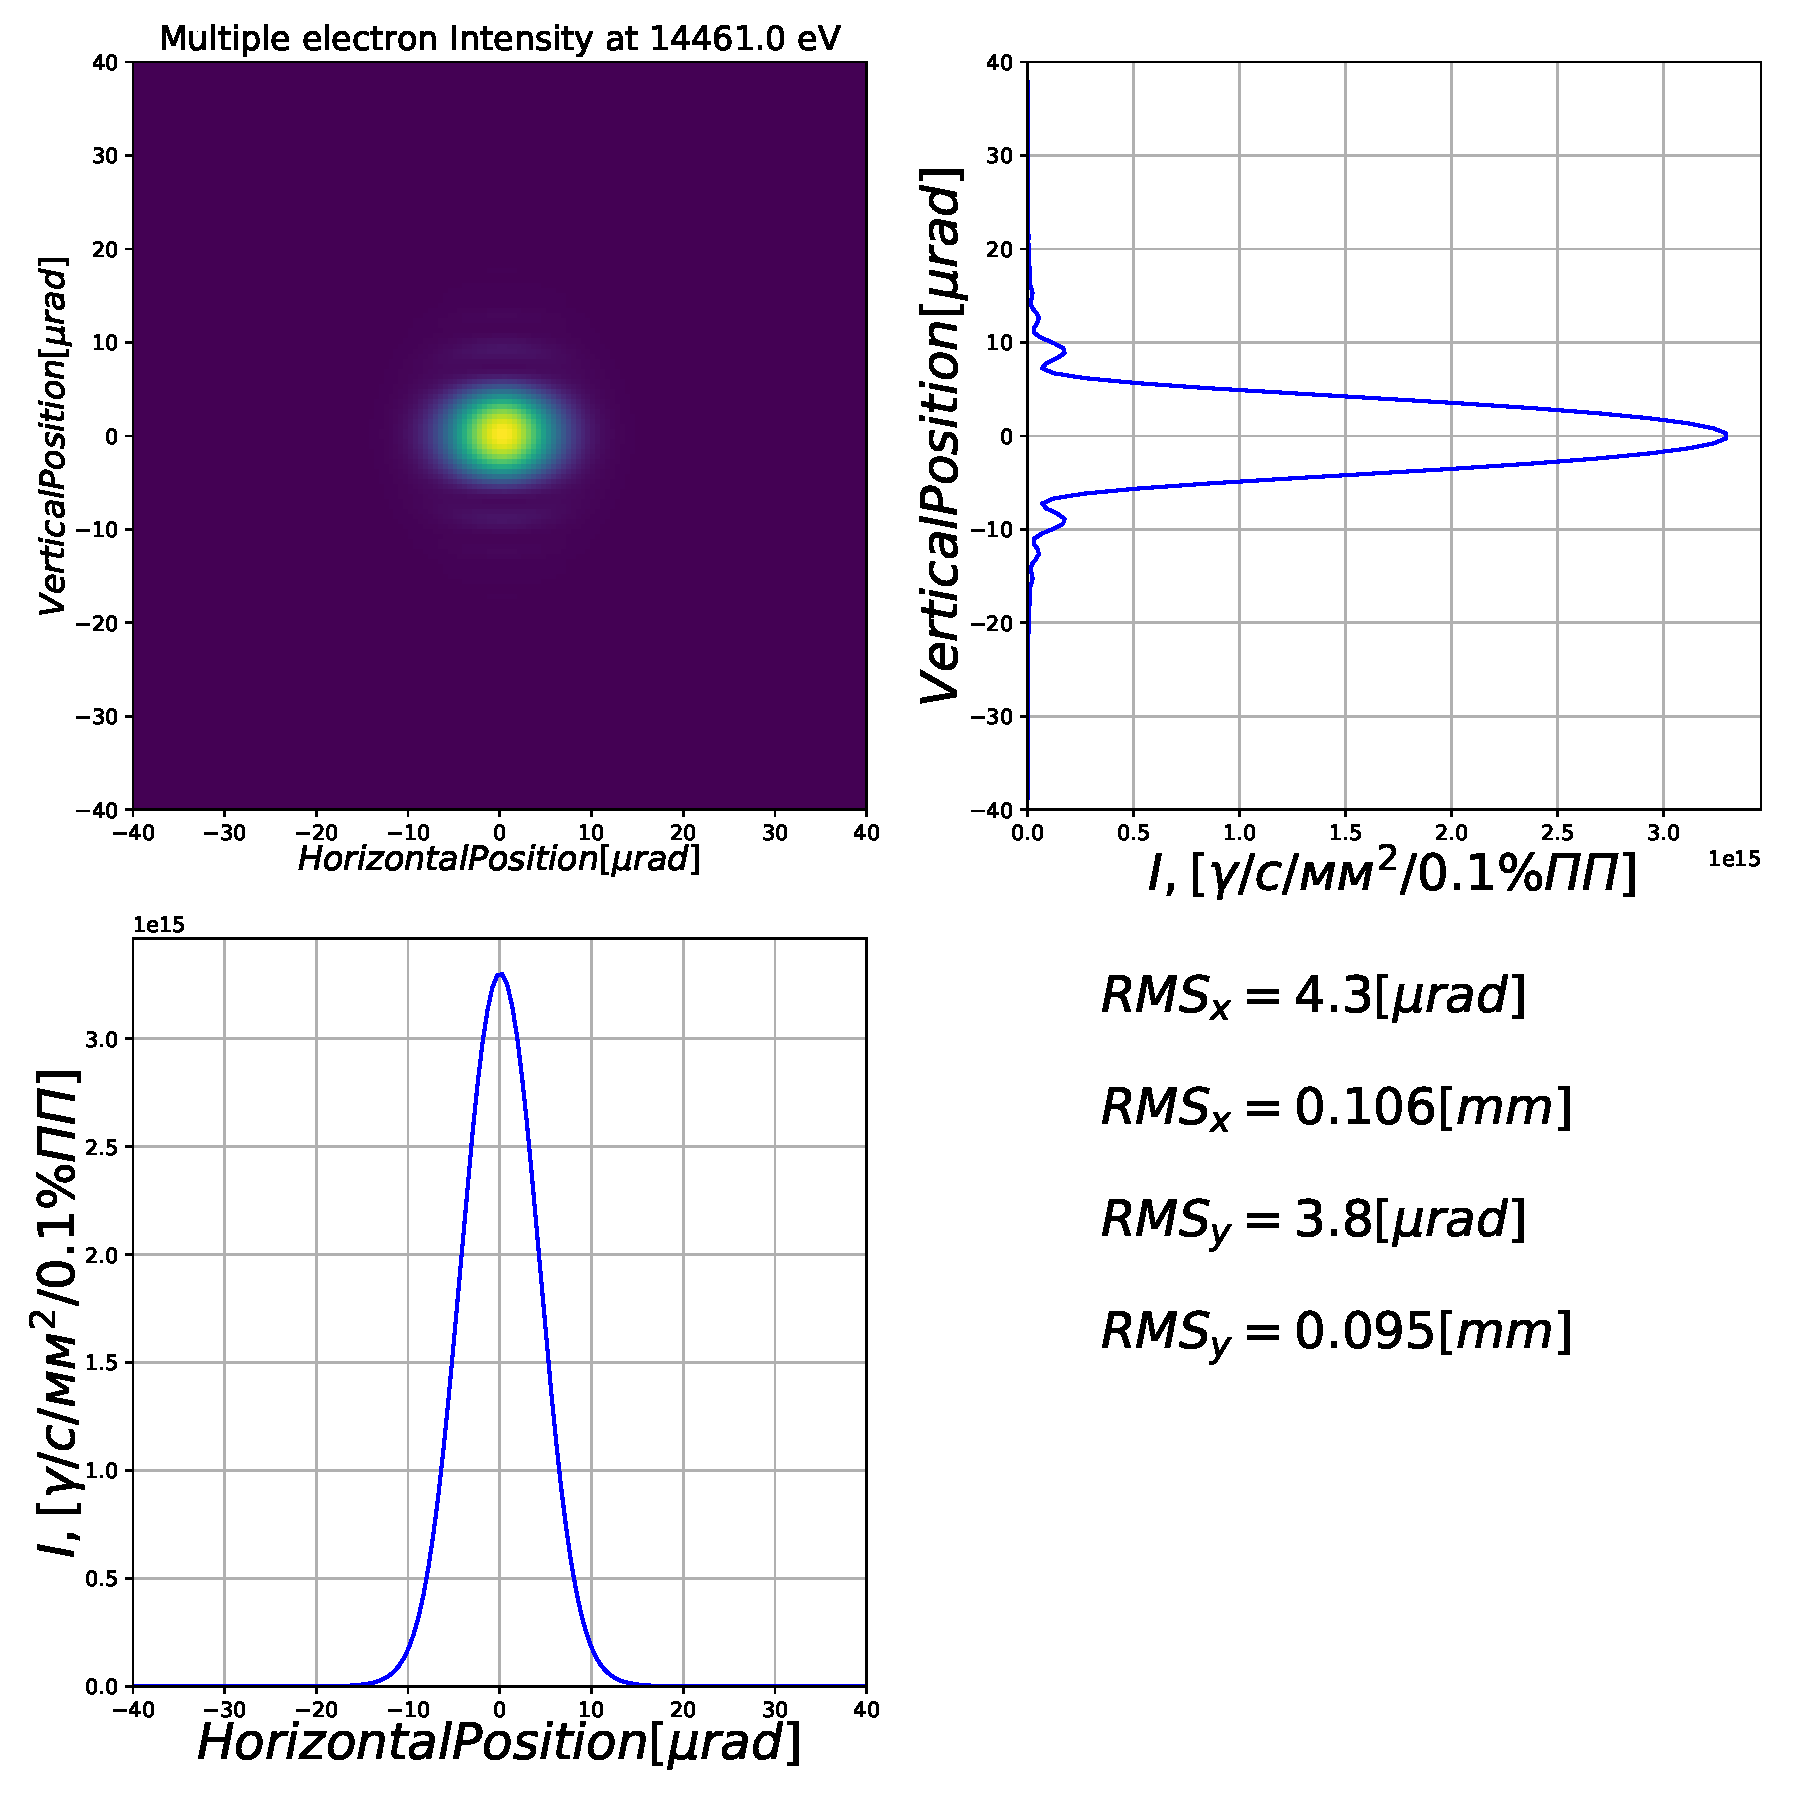
\includegraphics[width=\textwidth]{{pic/11_harm_before_crystal}.pdf}
	\end{minipage}\hfill
	\begin{minipage}{0.49\textwidth}
		\centering
		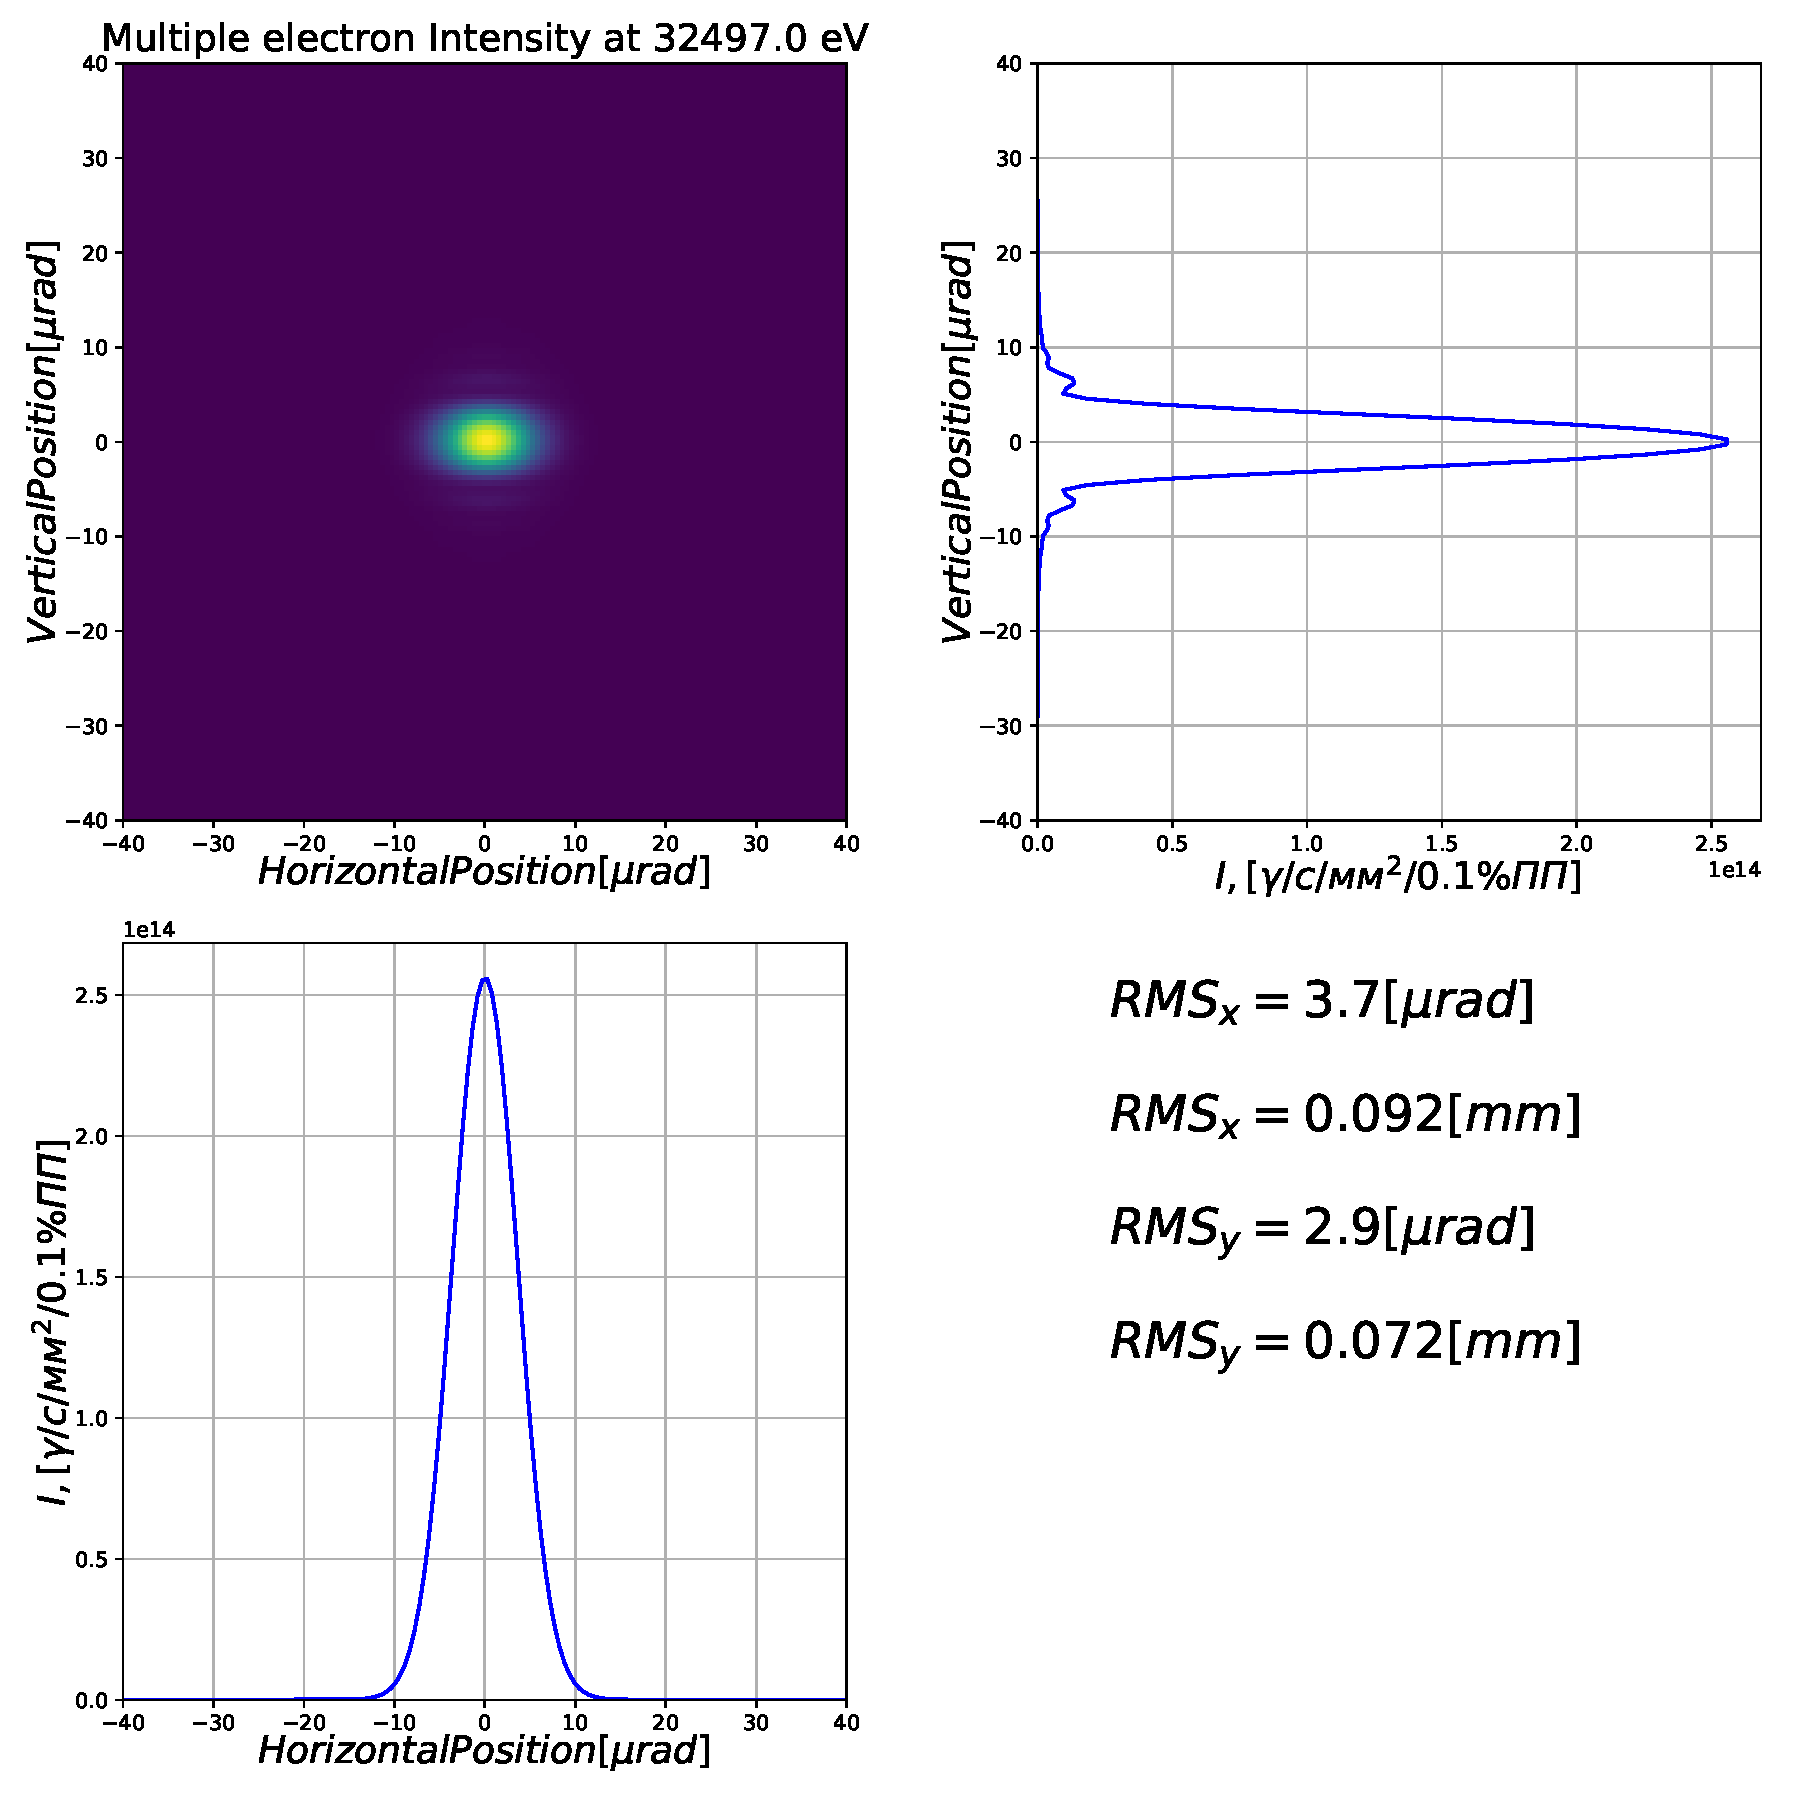
\includegraphics[width=\textwidth]{{pic/13_harm_before_crystal}.pdf}
	\end{minipage}
	\begin{minipage}{0.49\textwidth}
		\centering
		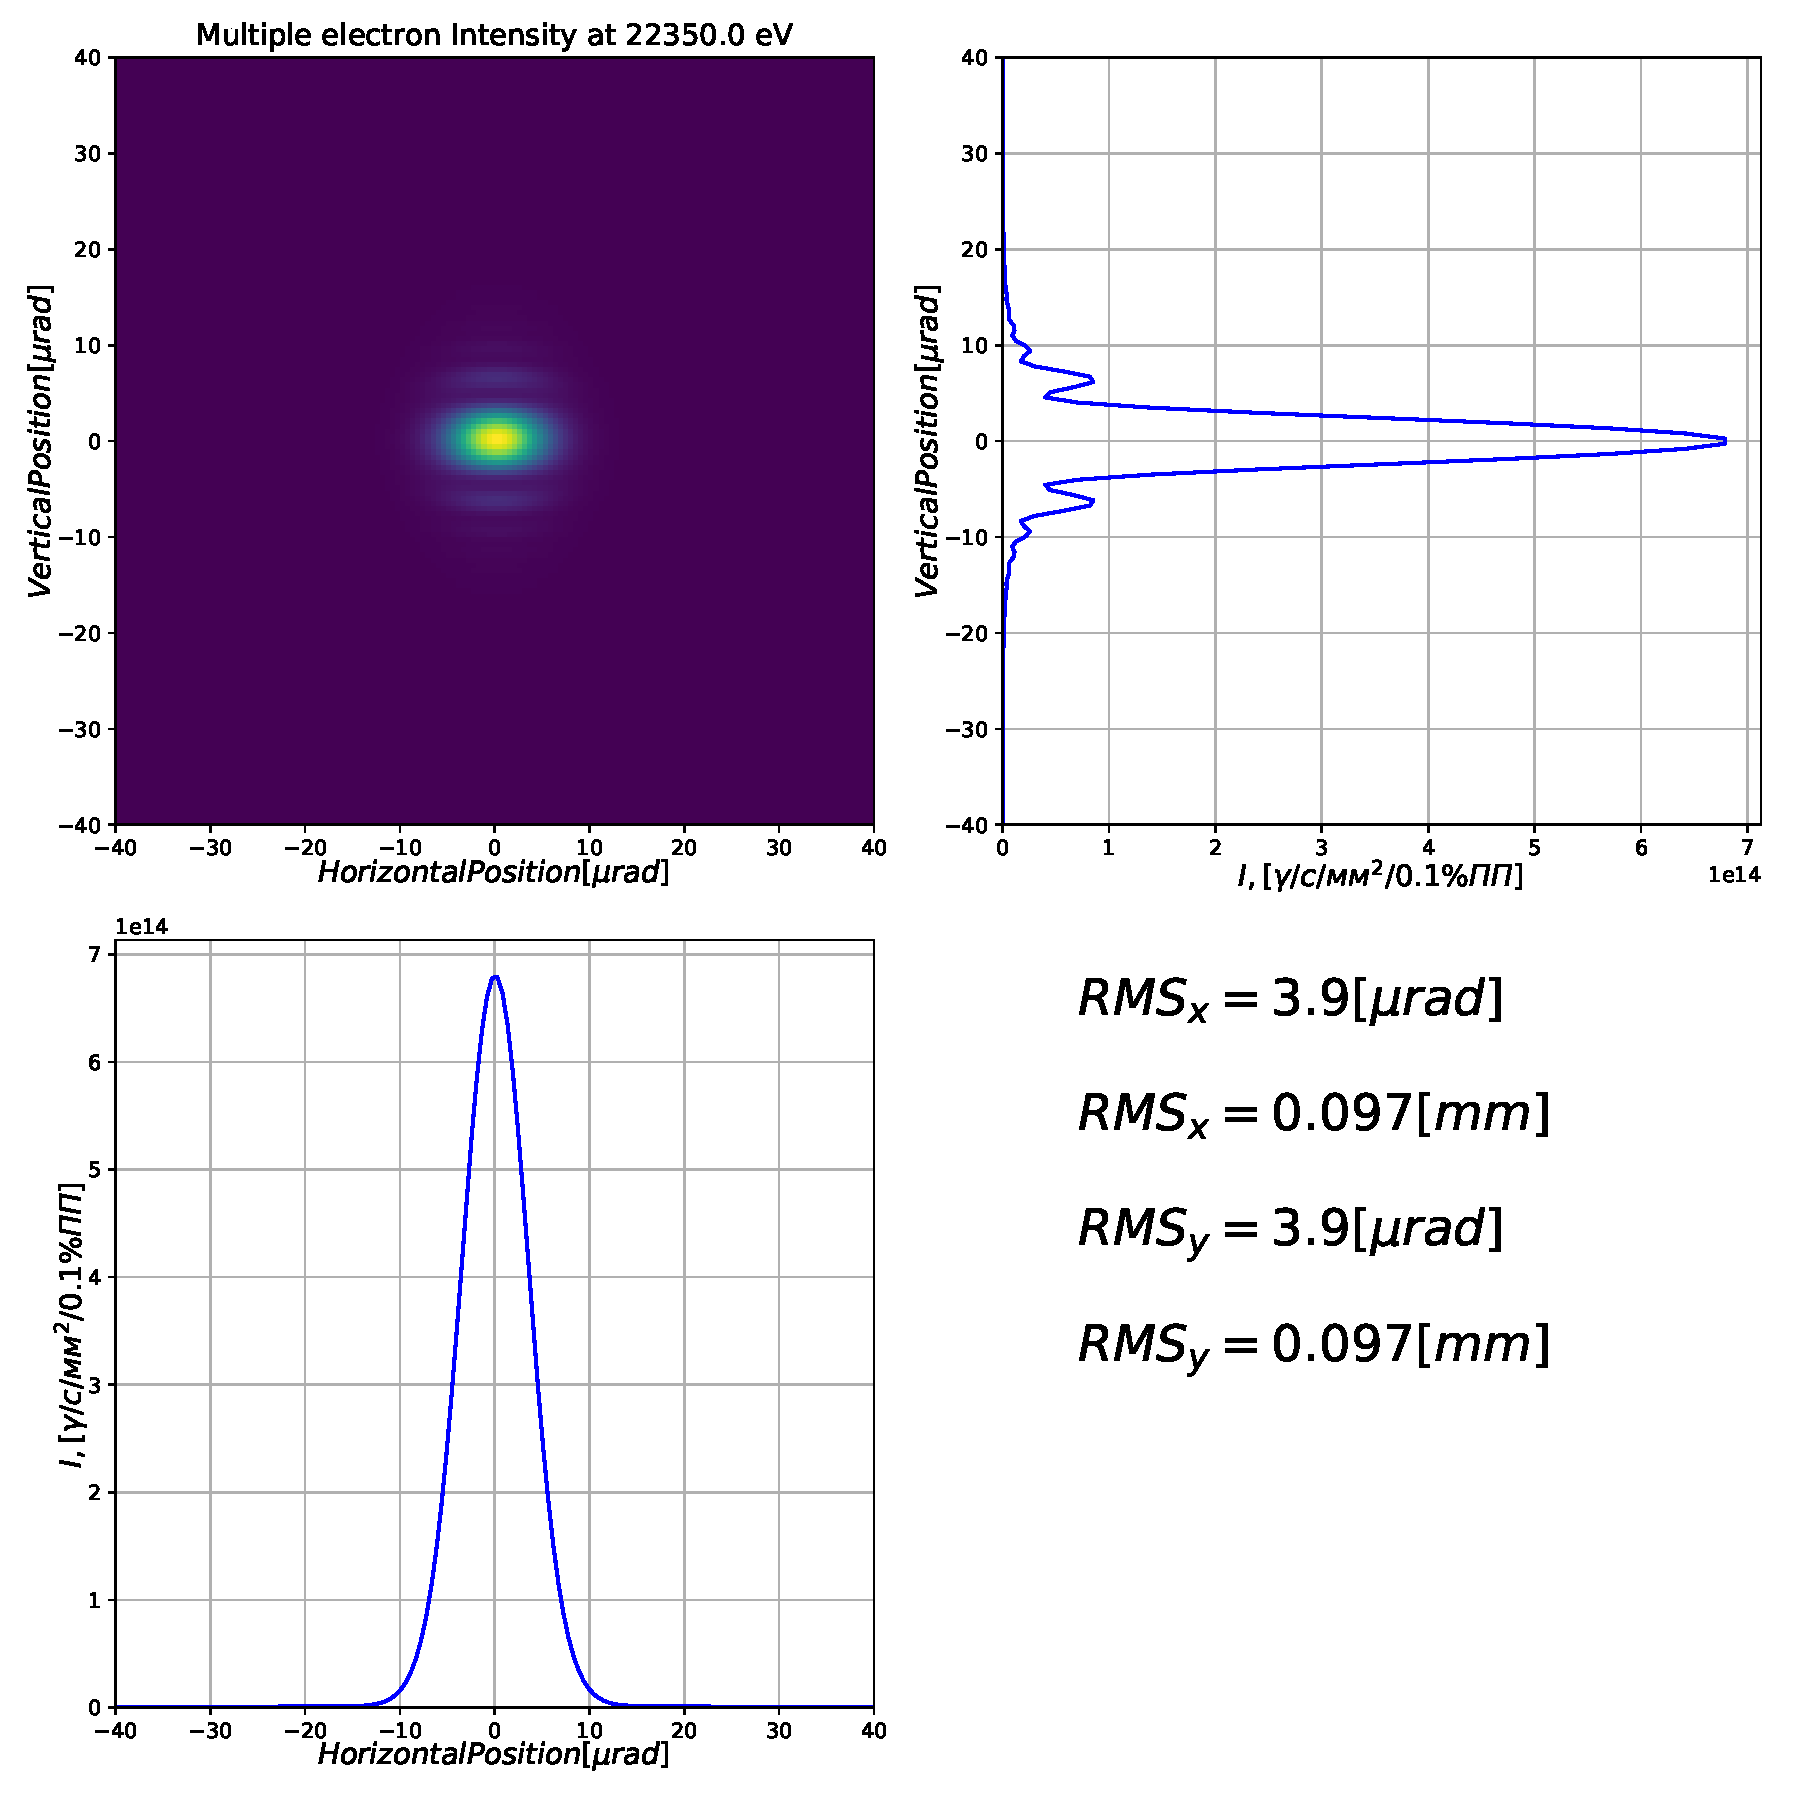
\includegraphics[width=\textwidth]{{pic/17_harm_before_crystal}.pdf}
	\end{minipage} 
	\begin{minipage}{0.49\textwidth}
		\centering
		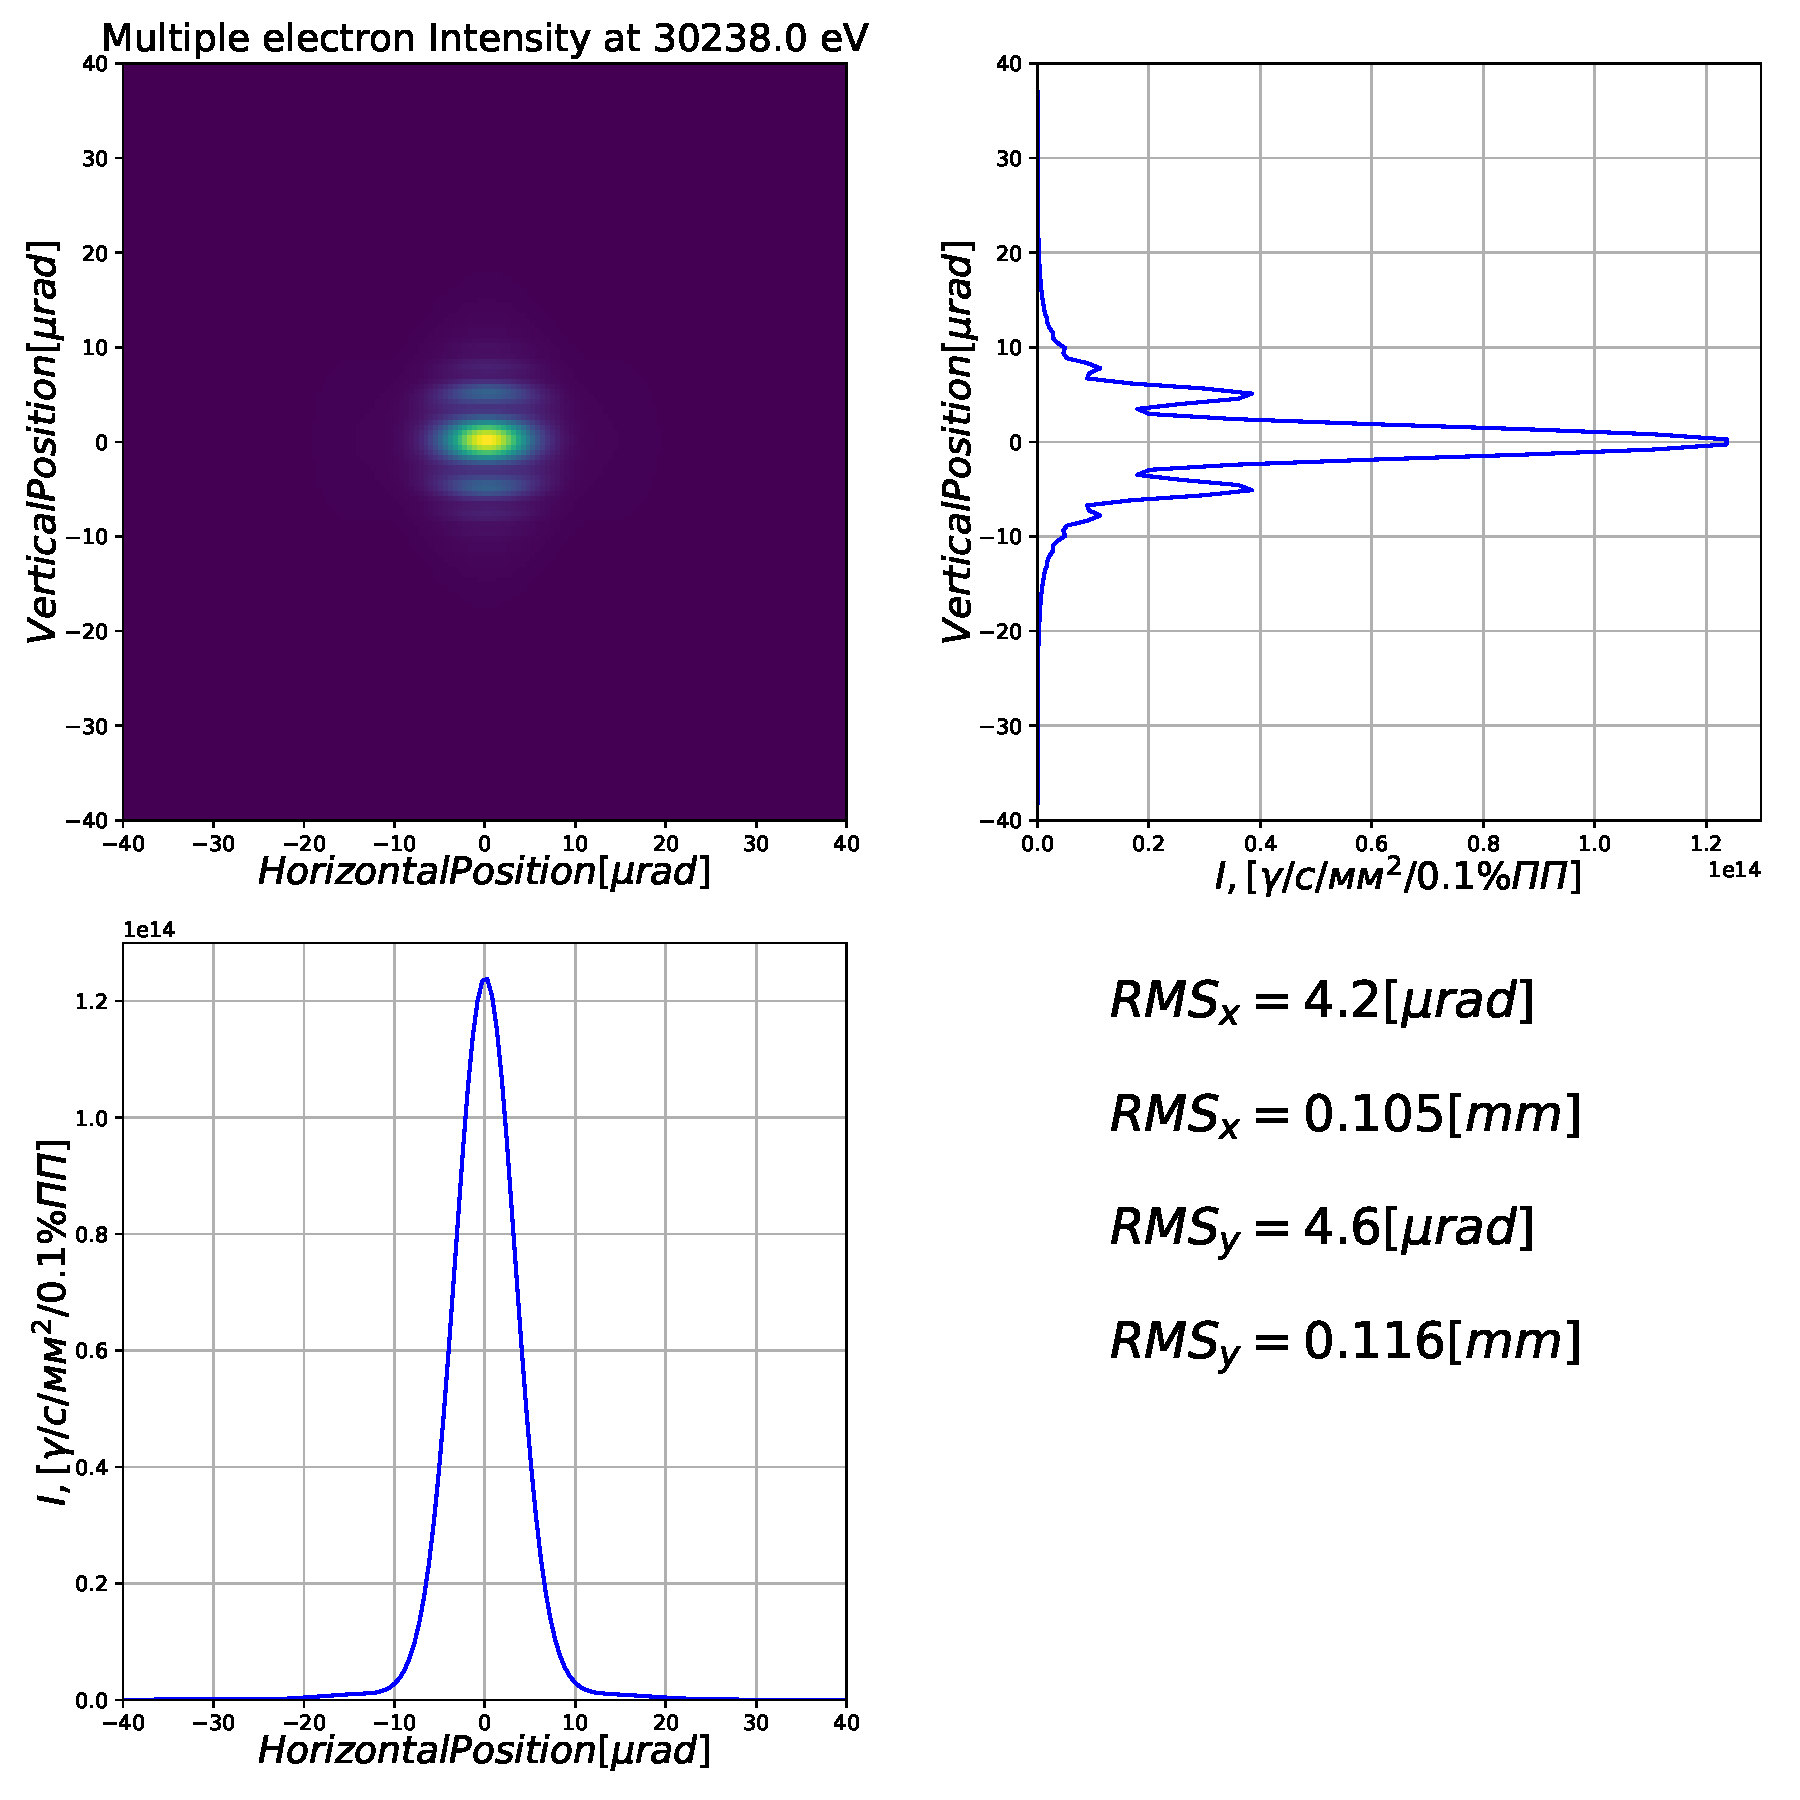
\includegraphics[width=\textwidth]{{pic/23_harm_before_crystal}.pdf}
	\end{minipage}
	\caption{Сечение пучка до первой аппретуры}    
	\label{fig:before_crystal}  
\end{figure}

\begin{figure}[htbp]
	\centering  
	\begin{minipage}{0.49\textwidth}
		\centering
		\includegraphics[width=\textwidth]{{pic/11_harm_after_crystal}.pdf}
	\end{minipage}\hfill
	\begin{minipage}{0.49\textwidth}
		\centering
		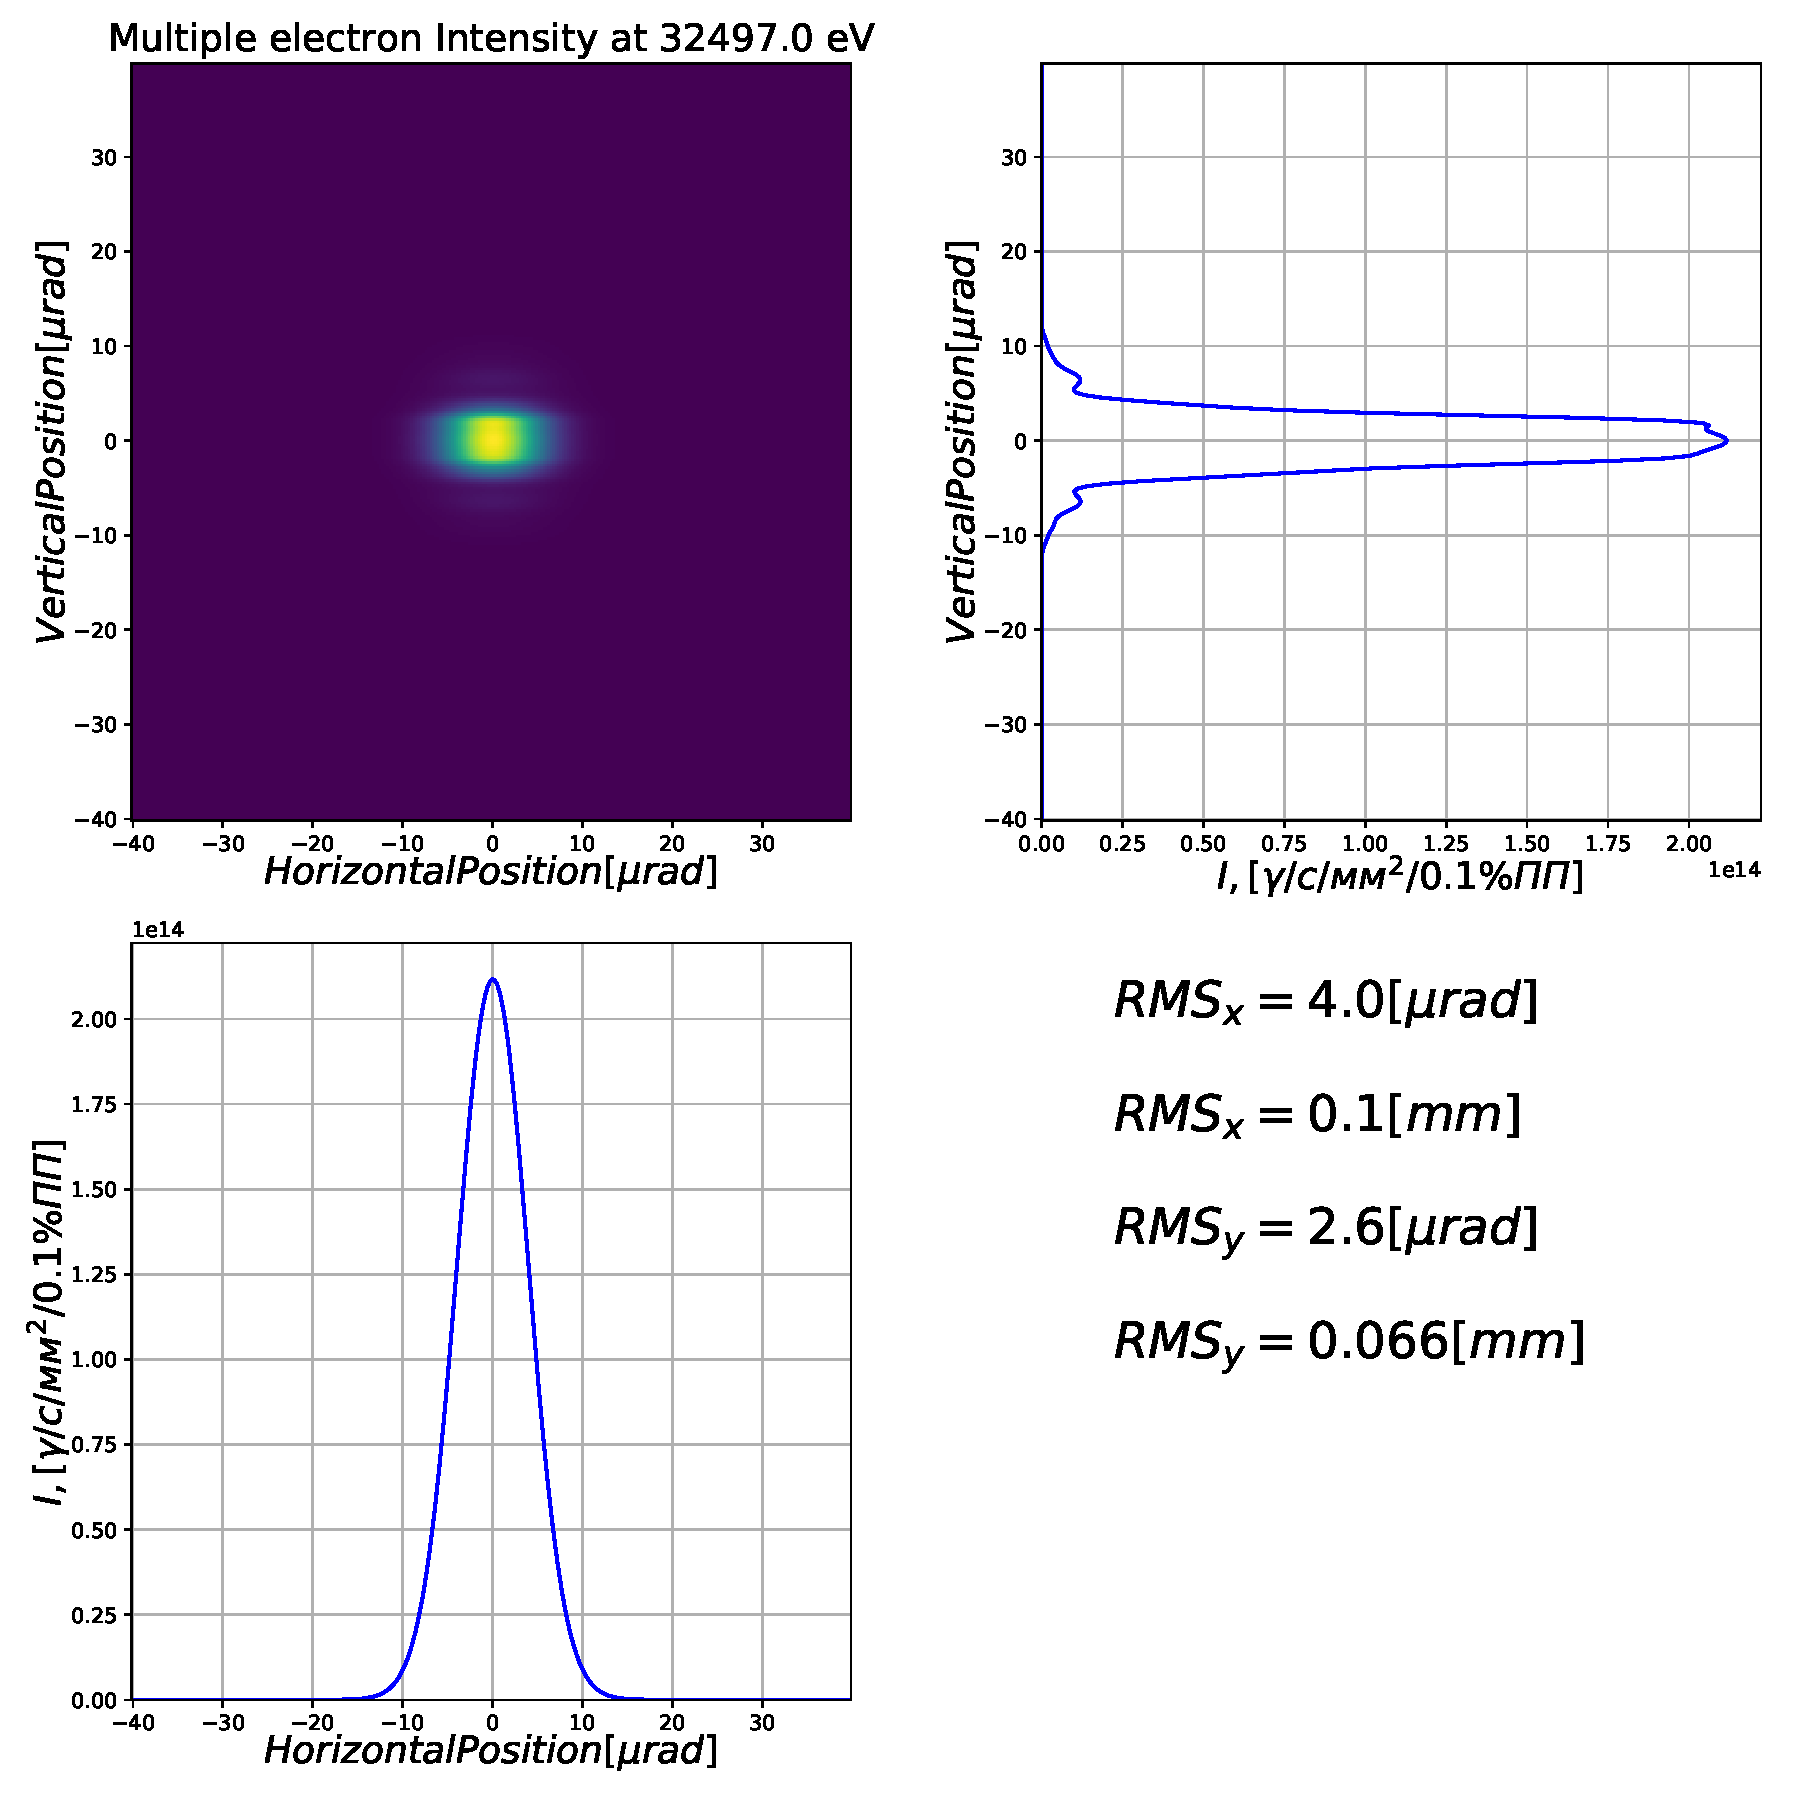
\includegraphics[width=\textwidth]{{pic/13_harm_after_crystal}.pdf}
	\end{minipage}
	\begin{minipage}{0.49\textwidth}
		\centering
		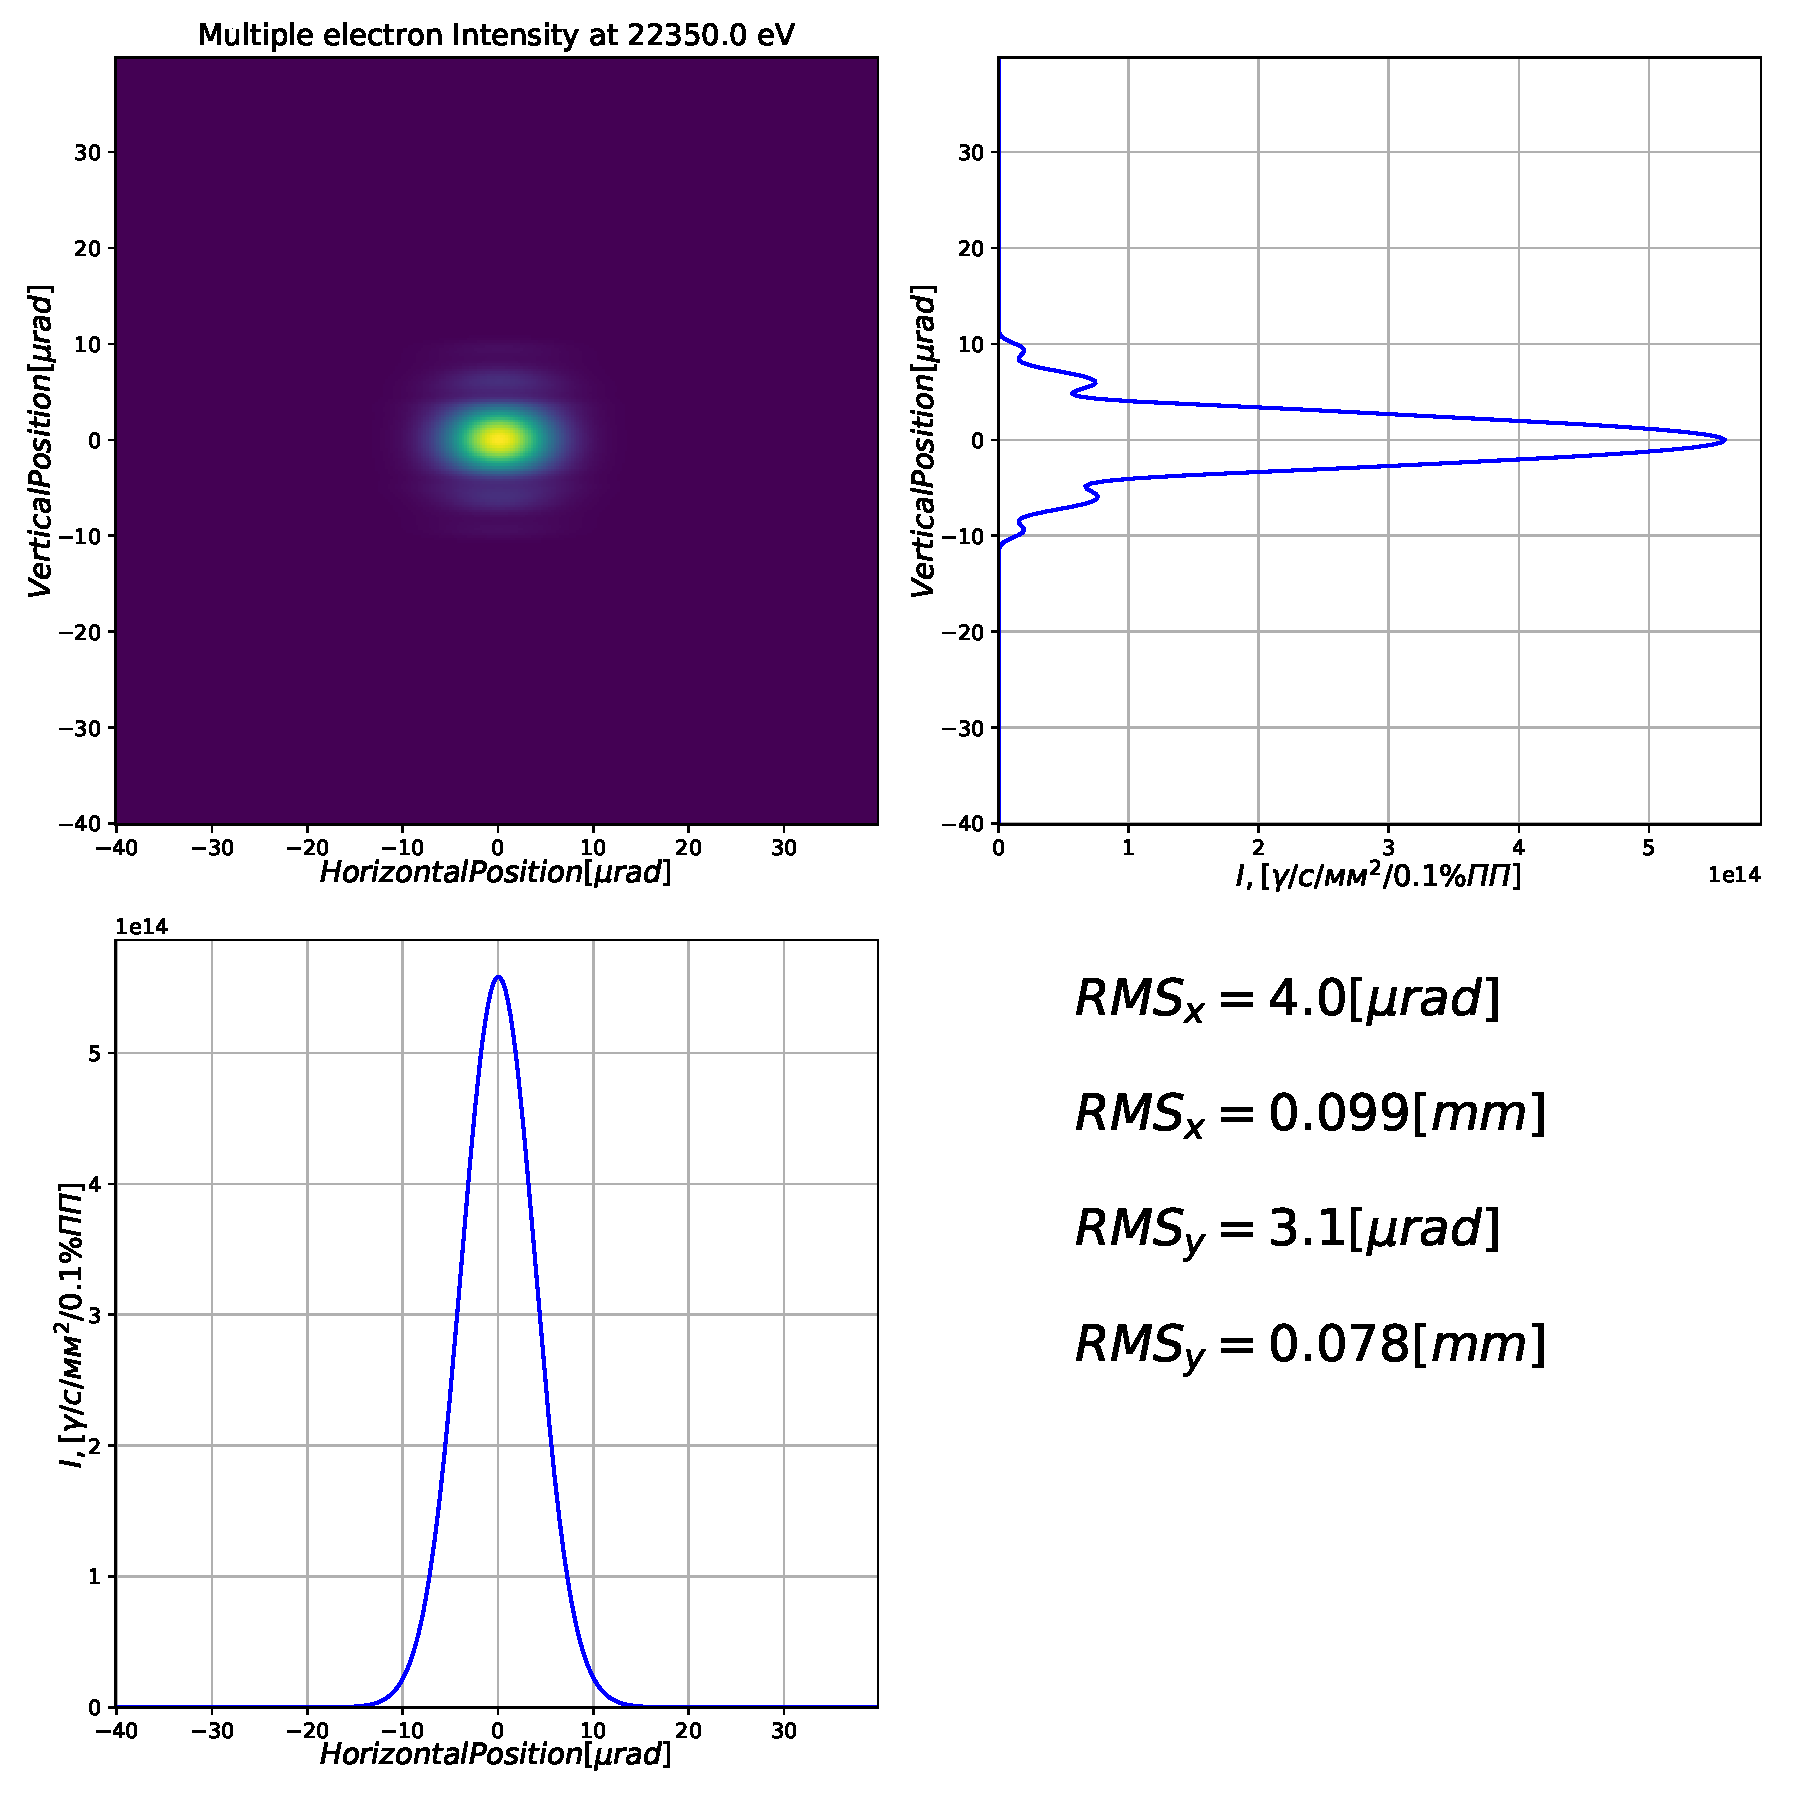
\includegraphics[width=\textwidth]{{pic/17_harm_after_crystal}.pdf}
		
	\end{minipage} 
	\begin{minipage}{0.49\textwidth}
		\centering
		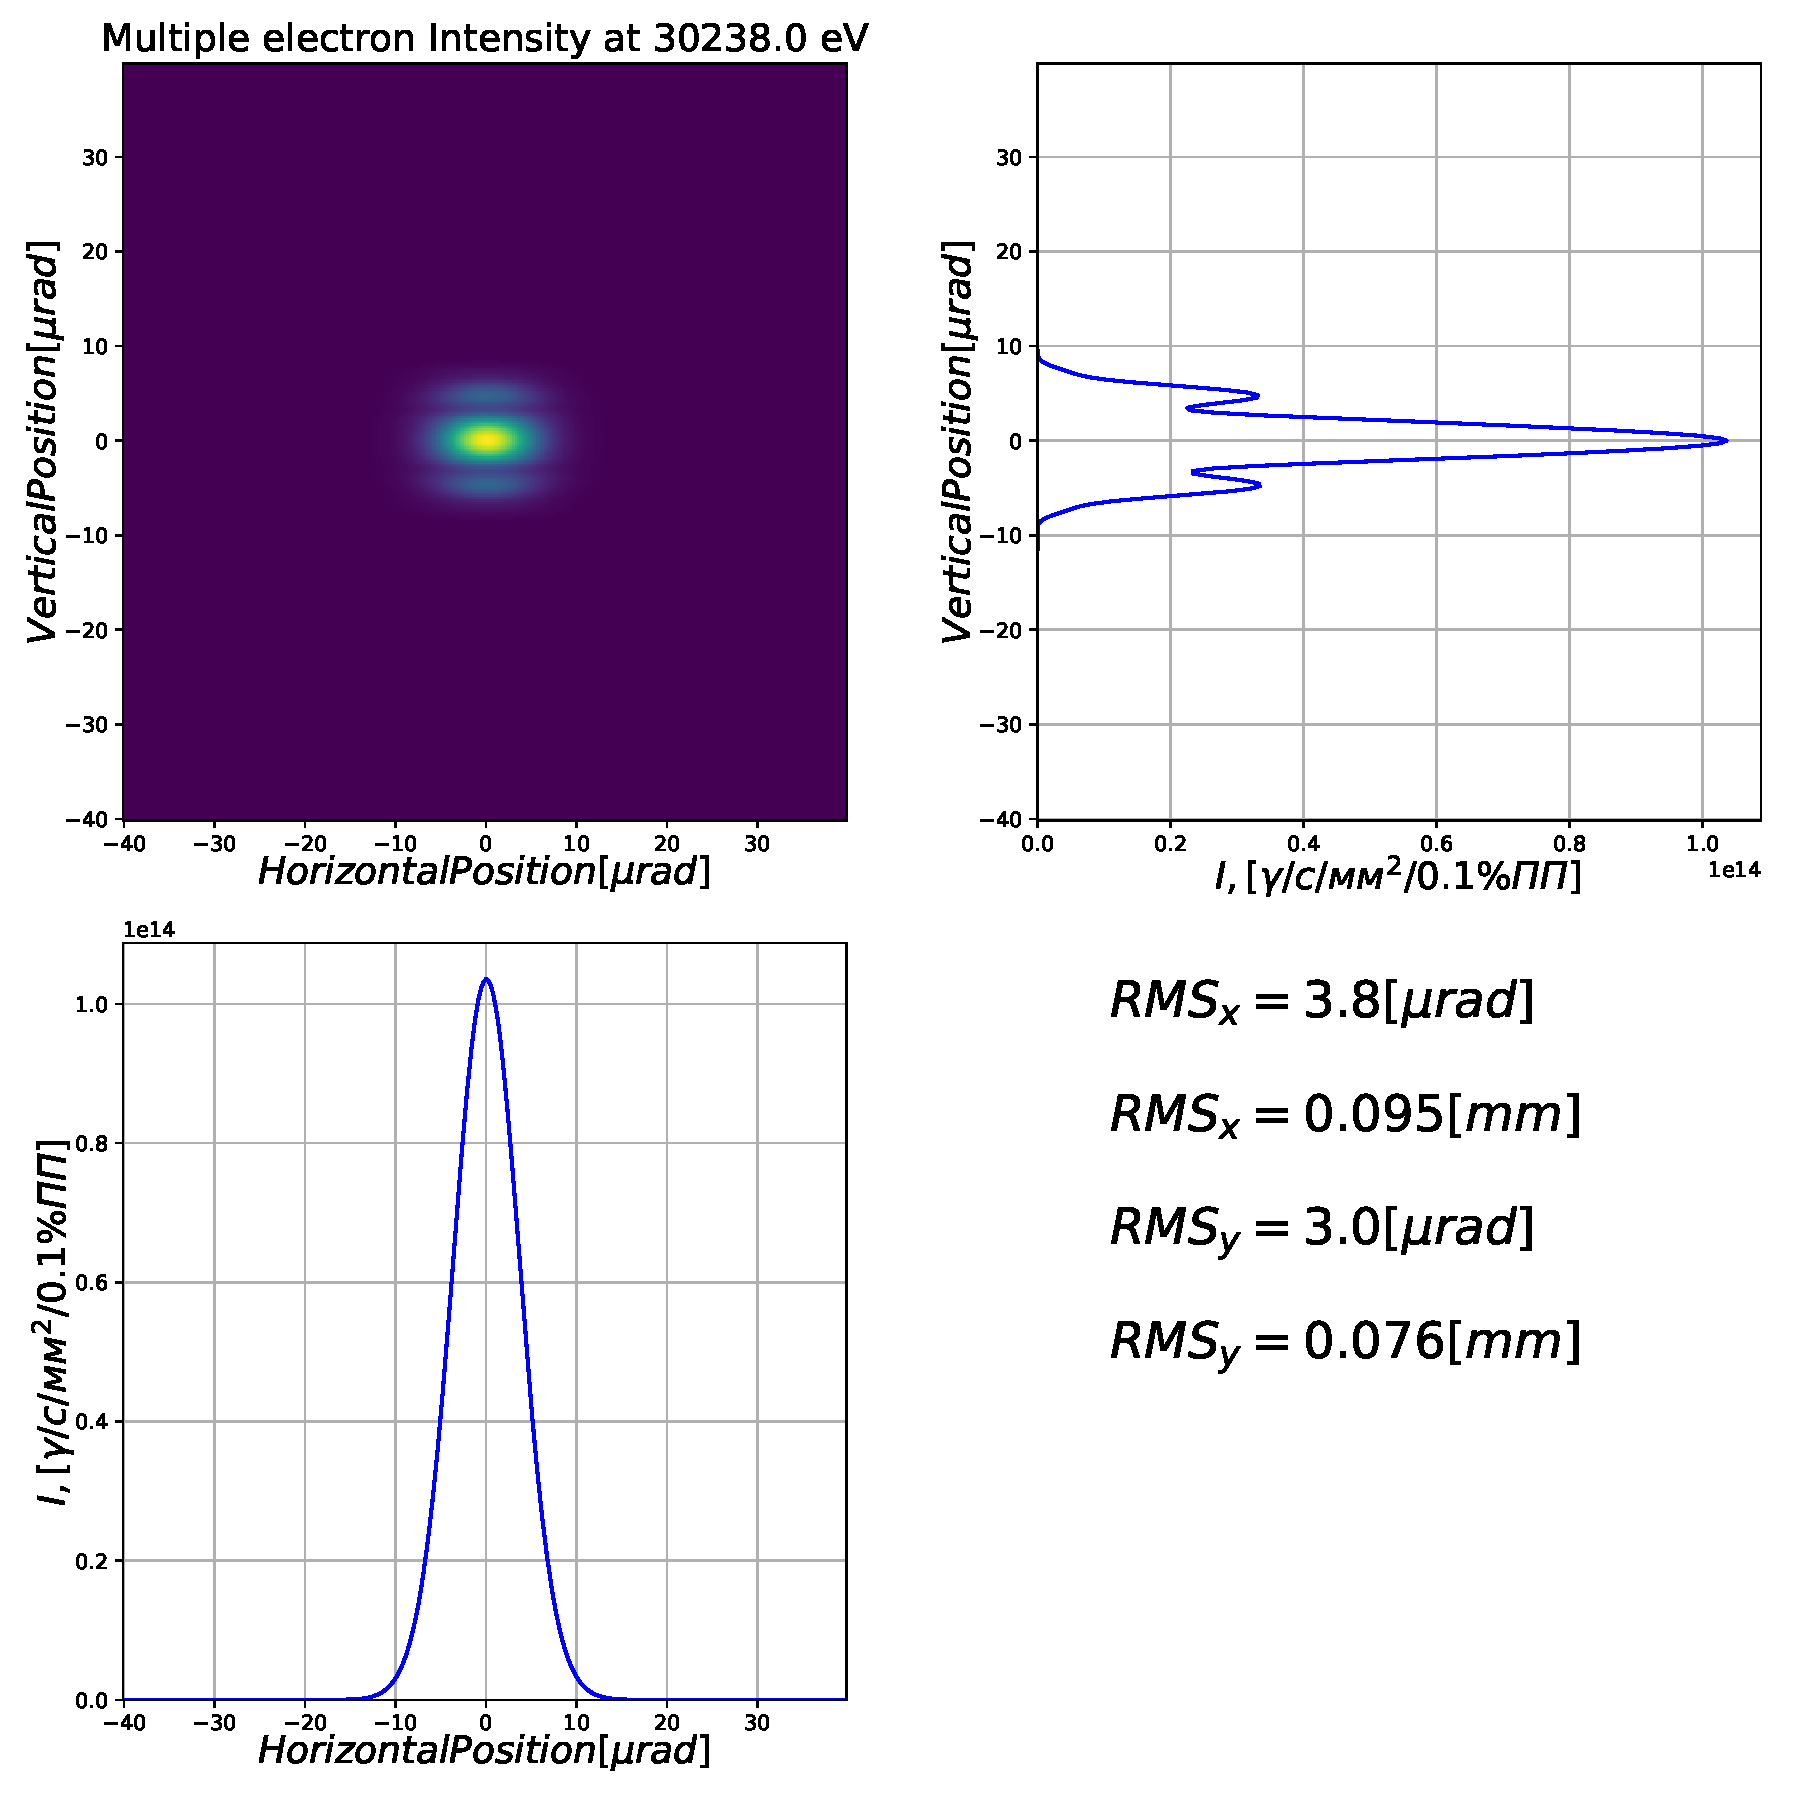
\includegraphics[width=\textwidth]{{pic/23_harm_after_crystal}.pdf}
	\end{minipage}
	\caption{Сечение пучка на выходе соответствующих монохроматоров}  
	\label{fig:after_crystal}  
\end{figure}

\end{document}







